\section{Demo và kết quả}

\subsection{Giao diện hỏi đáp}

\begin{figure}[htbp]
\centering
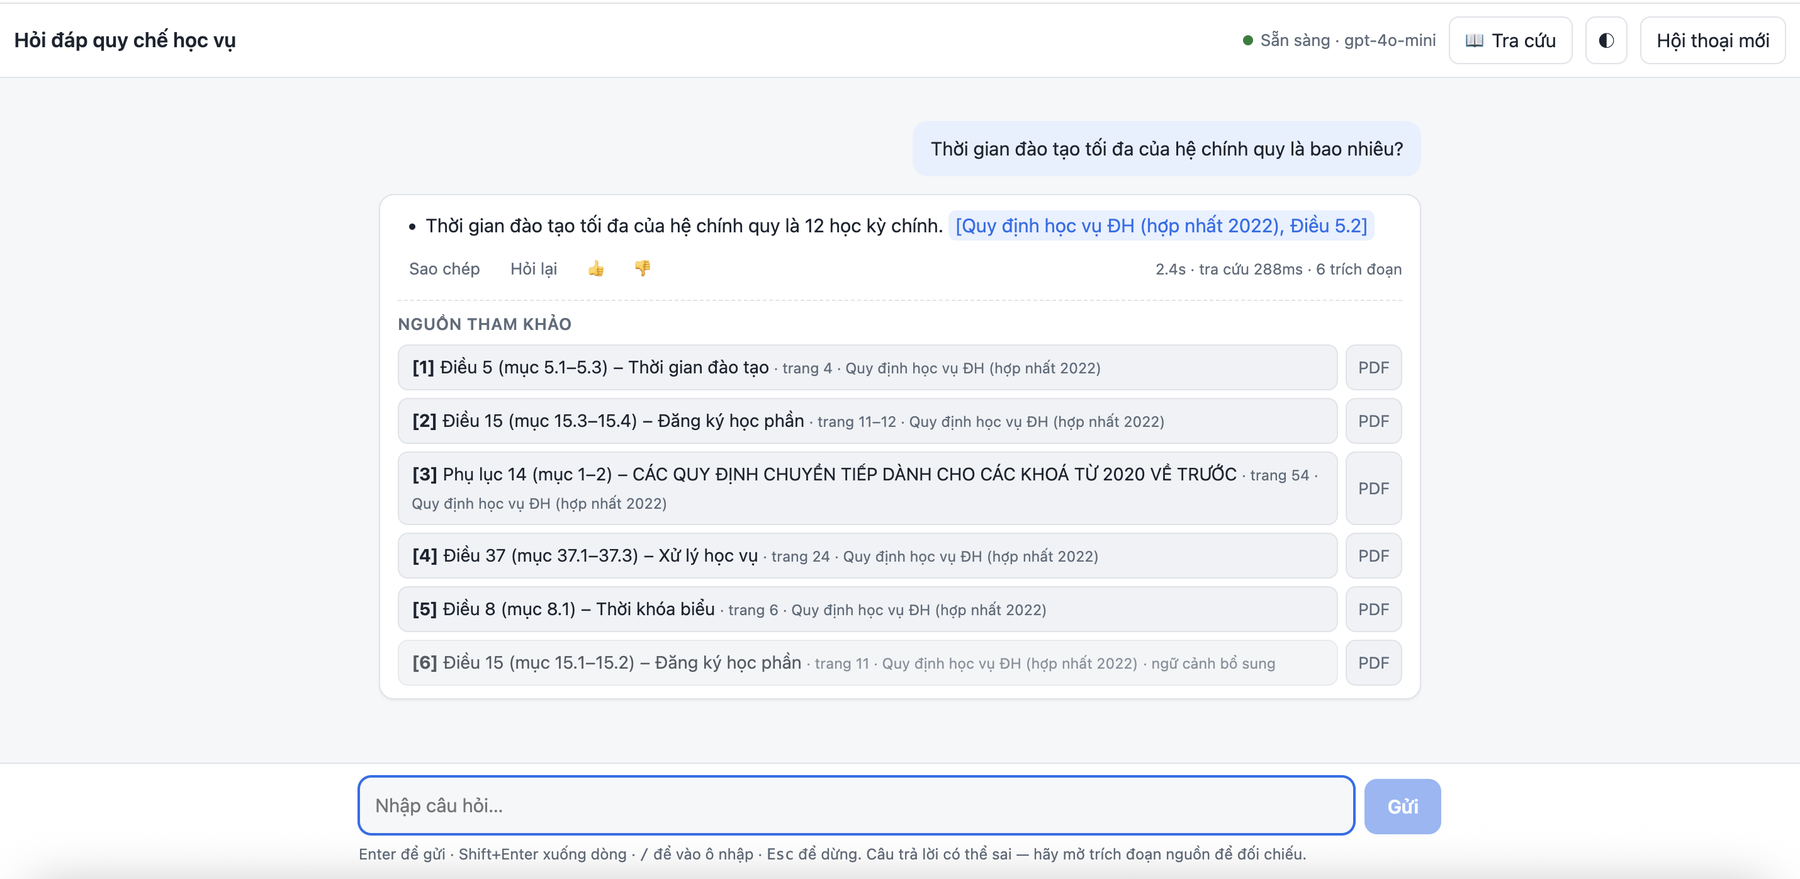
\includegraphics[width=\textwidth]{img/chat-demo.png}
\caption{Một lượt hỏi đáp. Trích dẫn \code{[Quy định học vụ ĐH (hợp nhất 2022), Điều 5.2]} được
tô nền và bấm được; dòng trạng thái cho biết tổng 2,4 giây, trong đó truy xuất 288\,ms.}
\label{fig:chat1}
\end{figure}

Câu trả lời đúng (12 học kỳ chính) và trích dẫn đúng tới khoản 5.2. Ảnh được chụp ở phiên bản
trước khi áp dụng ngưỡng liên quan theo từng trích đoạn, nên danh sách nguồn còn đủ sáu mục —
chính hiện tượng được mô tả ở mục~\ref{sec:nguong} và đã khắc phục
(xem hình~\ref{fig:count}).

\begin{figure}[htbp]
\centering
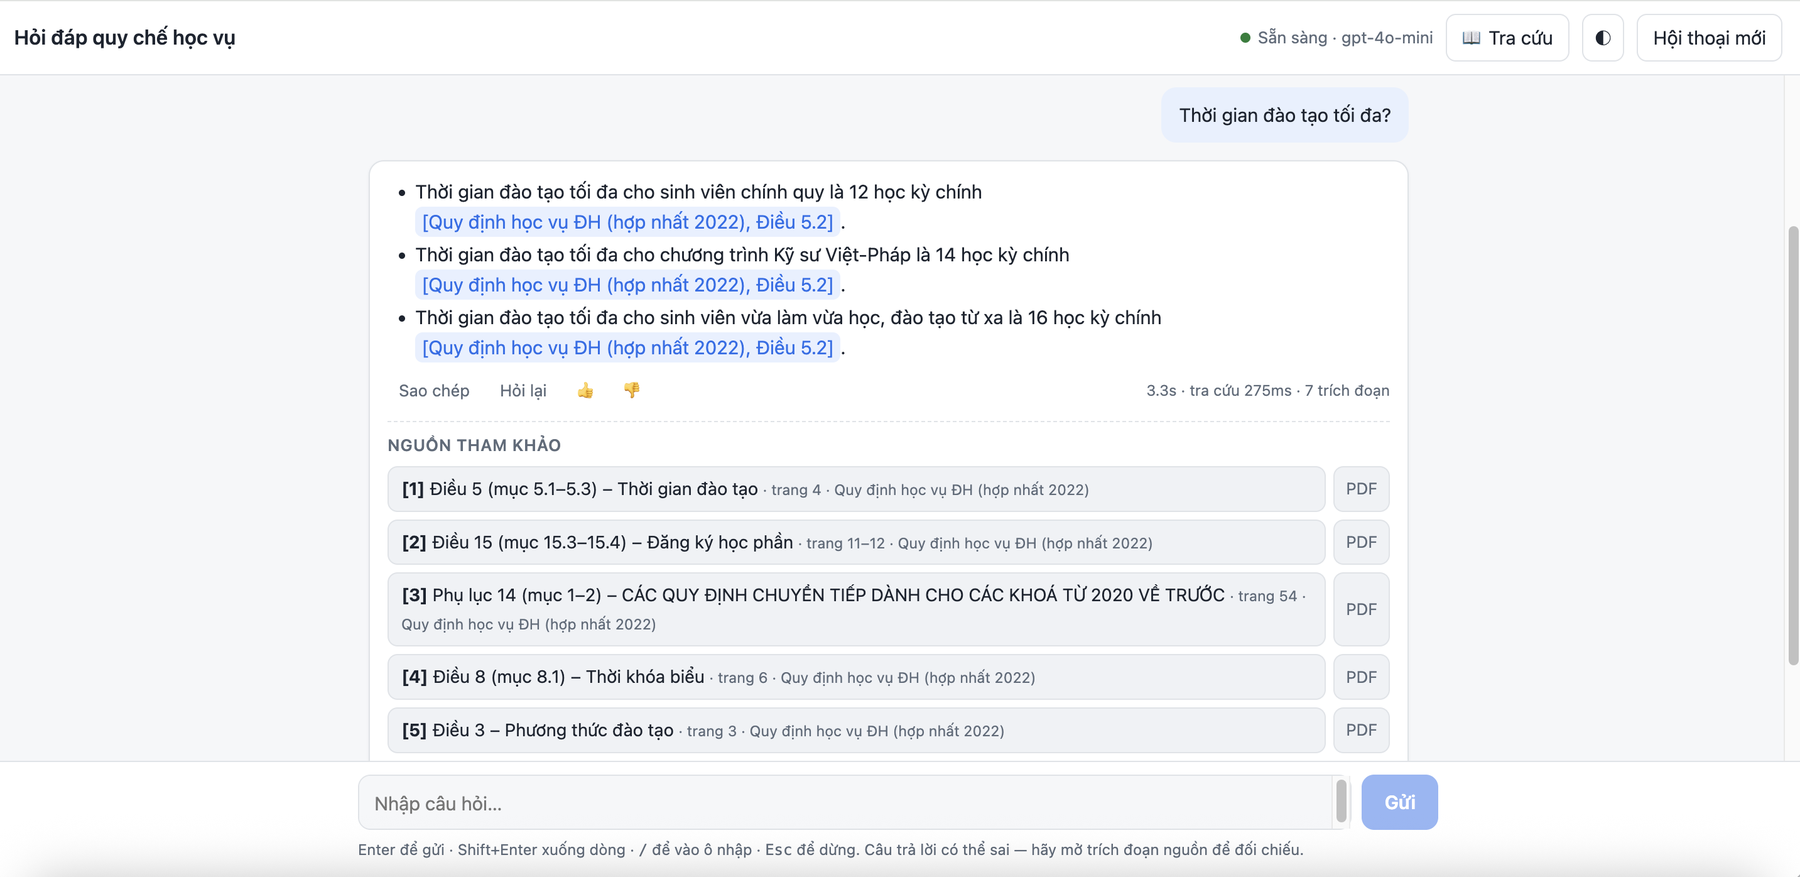
\includegraphics[width=\textwidth]{img/demo-chat-multi.png}
\caption{Khi quy định khác nhau theo đối tượng, prompt buộc mô hình nêu rõ từng trường hợp thay
vì gộp một con số: chính quy 12, Kỹ sư Việt-Pháp 14, vừa làm vừa học 16 học kỳ chính — đúng ba
dòng của bảng trong khoản 5.2.}
\label{fig:chat2}
\end{figure}

\begin{figure}[htbp]
\centering
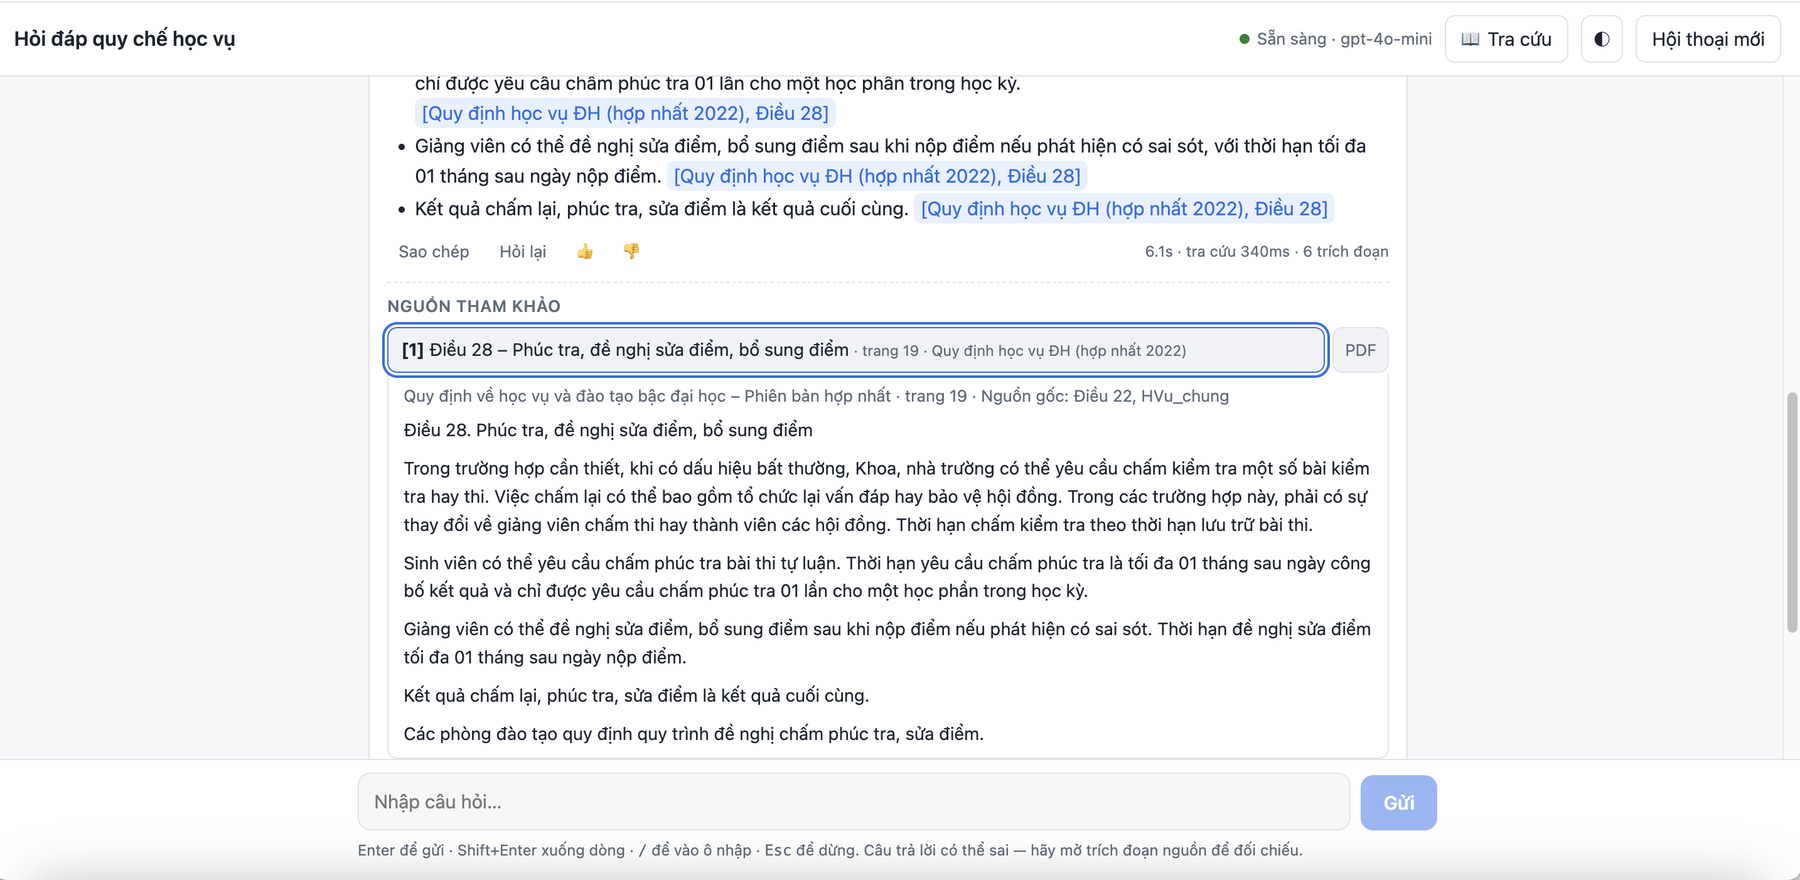
\includegraphics[width=\textwidth]{img/demo-source-open.png}
\caption{Bung một nguồn tham khảo. Toàn văn Điều 28 hiện ra kèm dòng xuất xứ “Nguồn gốc: Điều
22, HVu\_chung” — chú thích lề của bản hợp nhất, được OCR tách riêng và giữ lại suốt pipeline.
Người đọc đối chiếu được ngay mà không rời trang.}
\label{fig:source}
\end{figure}

\begin{figure}[htbp]
\centering
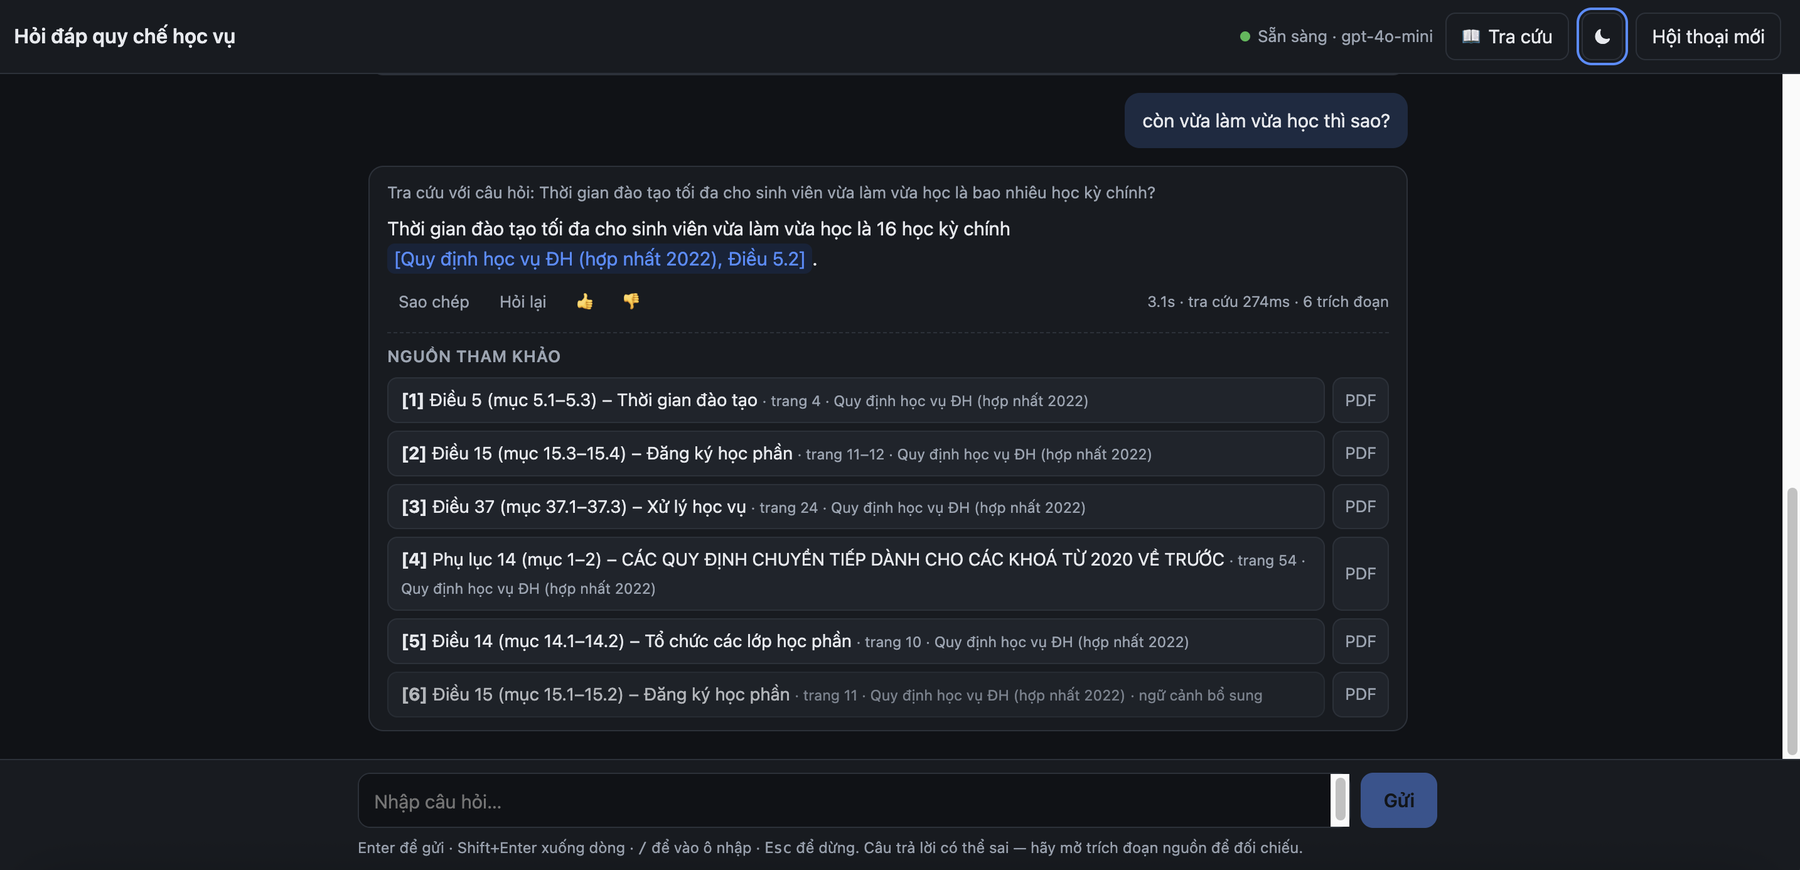
\includegraphics[width=\textwidth]{img/demo-dark-followup.png}
\caption{Câu hỏi nối tiếp “còn vừa làm vừa học thì sao?” được viết lại thành câu độc lập (dòng
xám phía trên) trước khi tra cứu, nên vẫn tìm đúng khoản 5.2 dù câu hỏi không nhắc tới thời
gian đào tạo. Ảnh cũng cho thấy chế độ giao diện tối.}
\label{fig:followup}
\end{figure}

\begin{figure}[htbp]
\centering
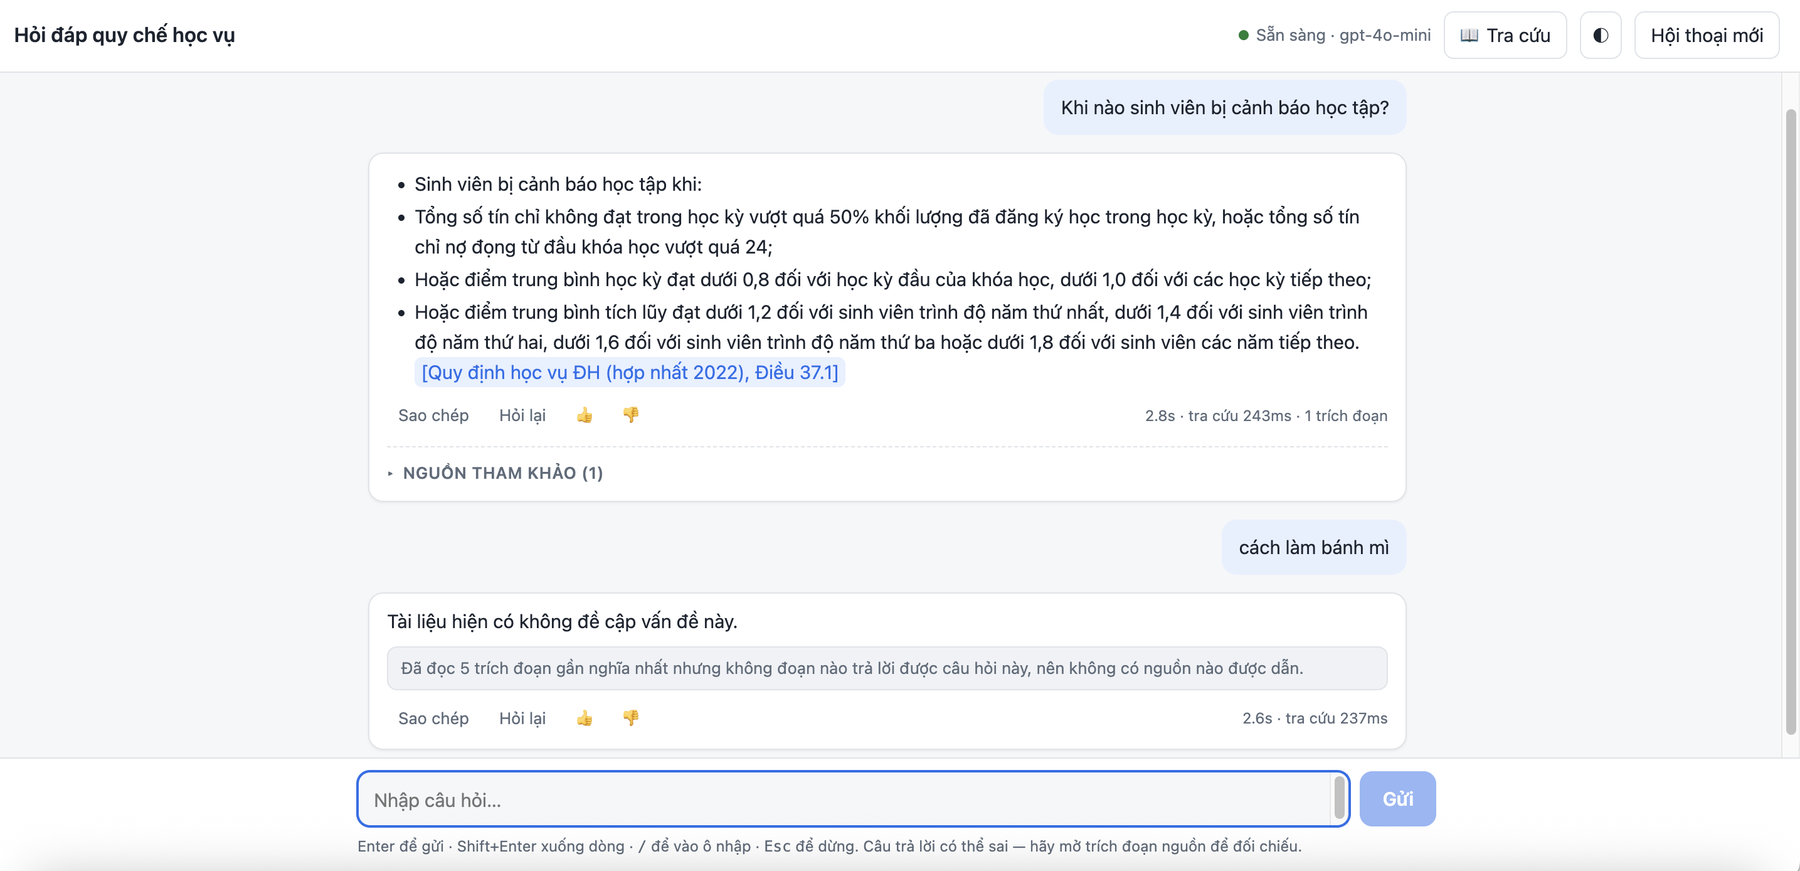
\includegraphics[width=\textwidth]{img/demo-count-refusal.png}
\caption{Hai hành vi trong một màn hình. Câu hỏi về cảnh báo học tập được trả lời bằng
\textbf{đúng một} trích đoạn, vì ngưỡng liên quan theo từng trích đoạn
(mục~\ref{sec:nguong}) đã loại phần còn lại. Câu hỏi ngoài phạm vi phía dưới nhận một lời từ
chối, kèm dòng giải thích đã đọc bao nhiêu trích đoạn và vì sao không dẫn nguồn nào.}
\label{fig:count}
\end{figure}

\begin{figure}[htbp]
\centering
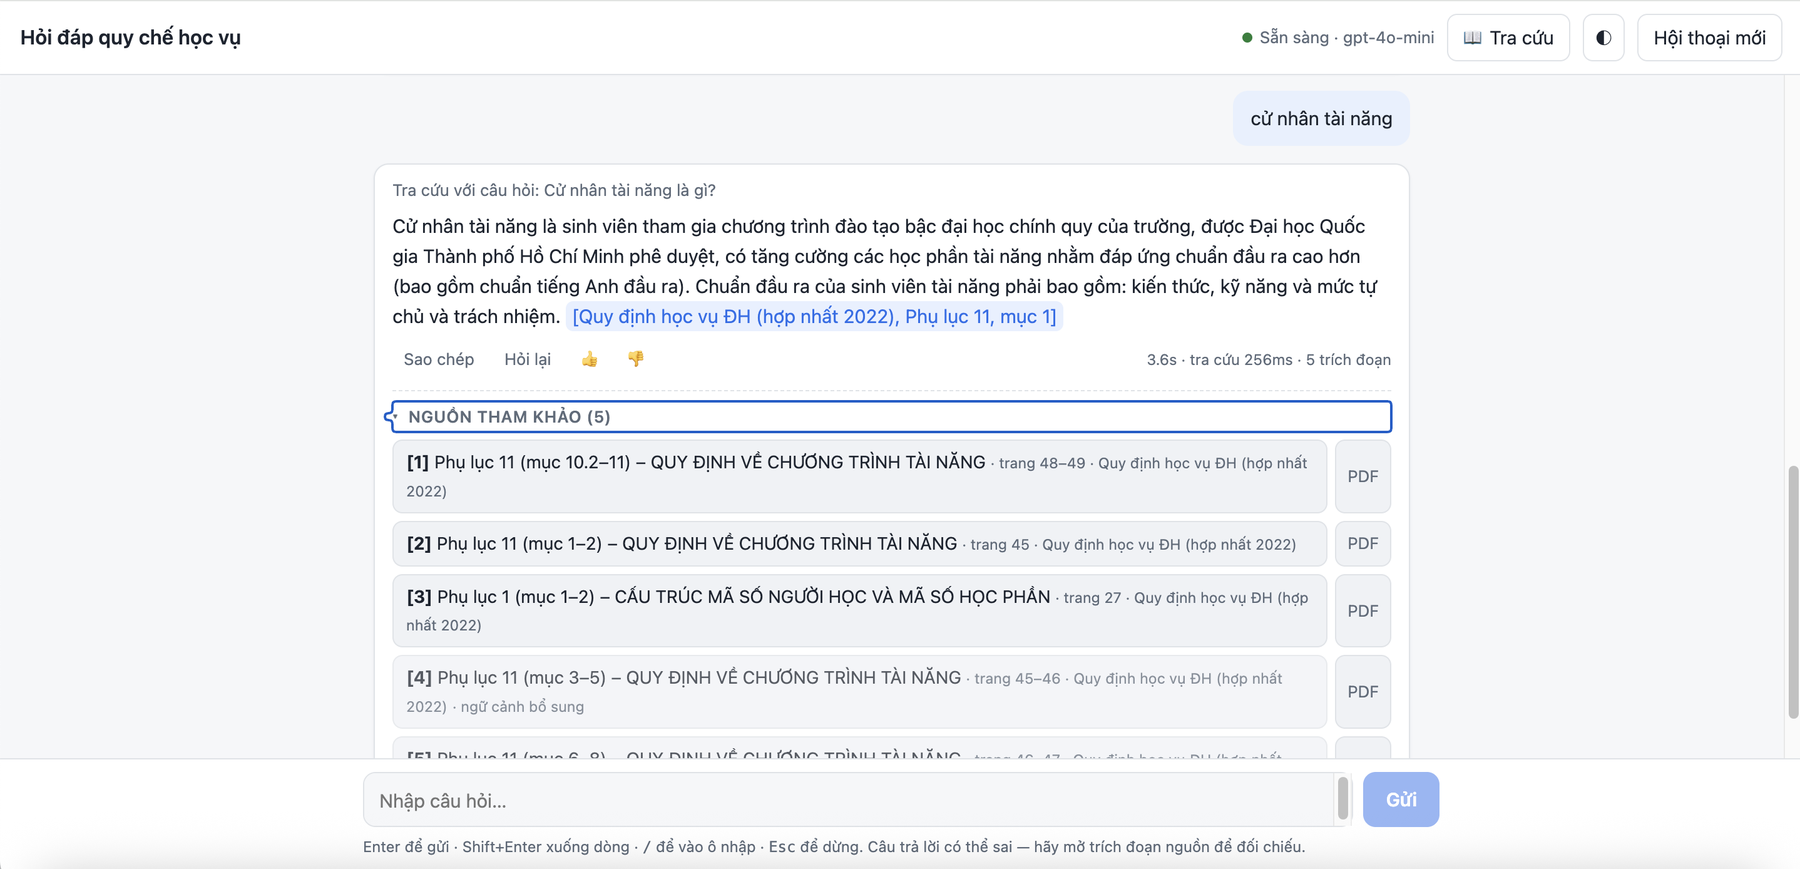
\includegraphics[width=\textwidth]{img/demo-sources-open-5.png}
\caption{Cùng giao diện, câu hỏi rộng hơn: năm trích đoạn vượt ngưỡng, và người đọc đã bấm bung
danh sách. Trích dẫn trỏ tới một Phụ lục thay vì một Điều, và câu hỏi hai từ “cử nhân tài năng”
được viết lại thành câu hoàn chỉnh trước khi tra cứu.}
\label{fig:open5}
\end{figure}

\subsection{Trang tra cứu toàn văn}

\begin{figure}[htbp]
\centering
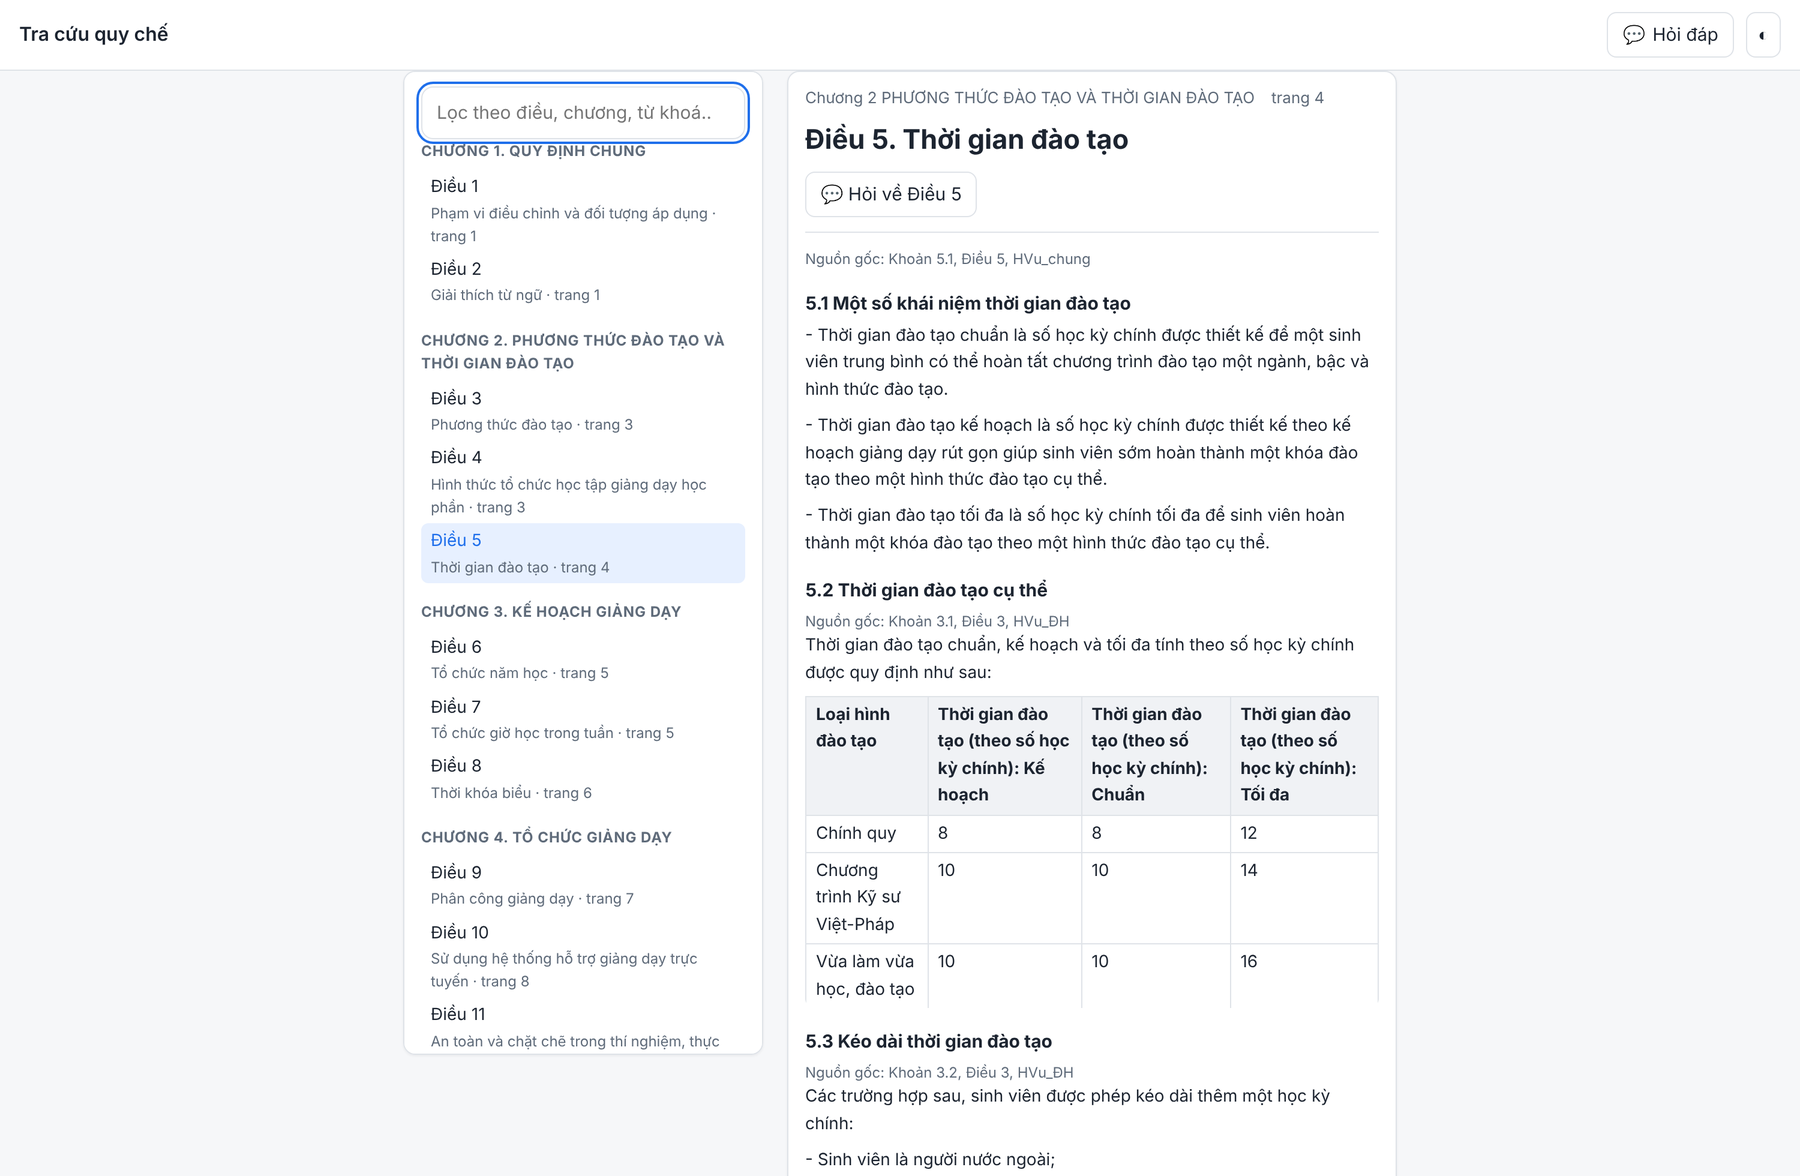
\includegraphics[width=\textwidth]{img/browse-dieu5.png}
\caption{Trang tra cứu. Mục lục bên trái dựng trực tiếp từ Markdown đã được nạp nên không bao
giờ lệch với dữ liệu đã đánh chỉ mục. Bảng “thời gian đào tạo” được dựng lại thành bảng HTML,
và mỗi khoản hiện chú thích nguồn gốc riêng.}
\label{fig:browse}
\end{figure}

\subsection{Trang chẩn đoán truy xuất}

\begin{figure}[htbp]
\centering
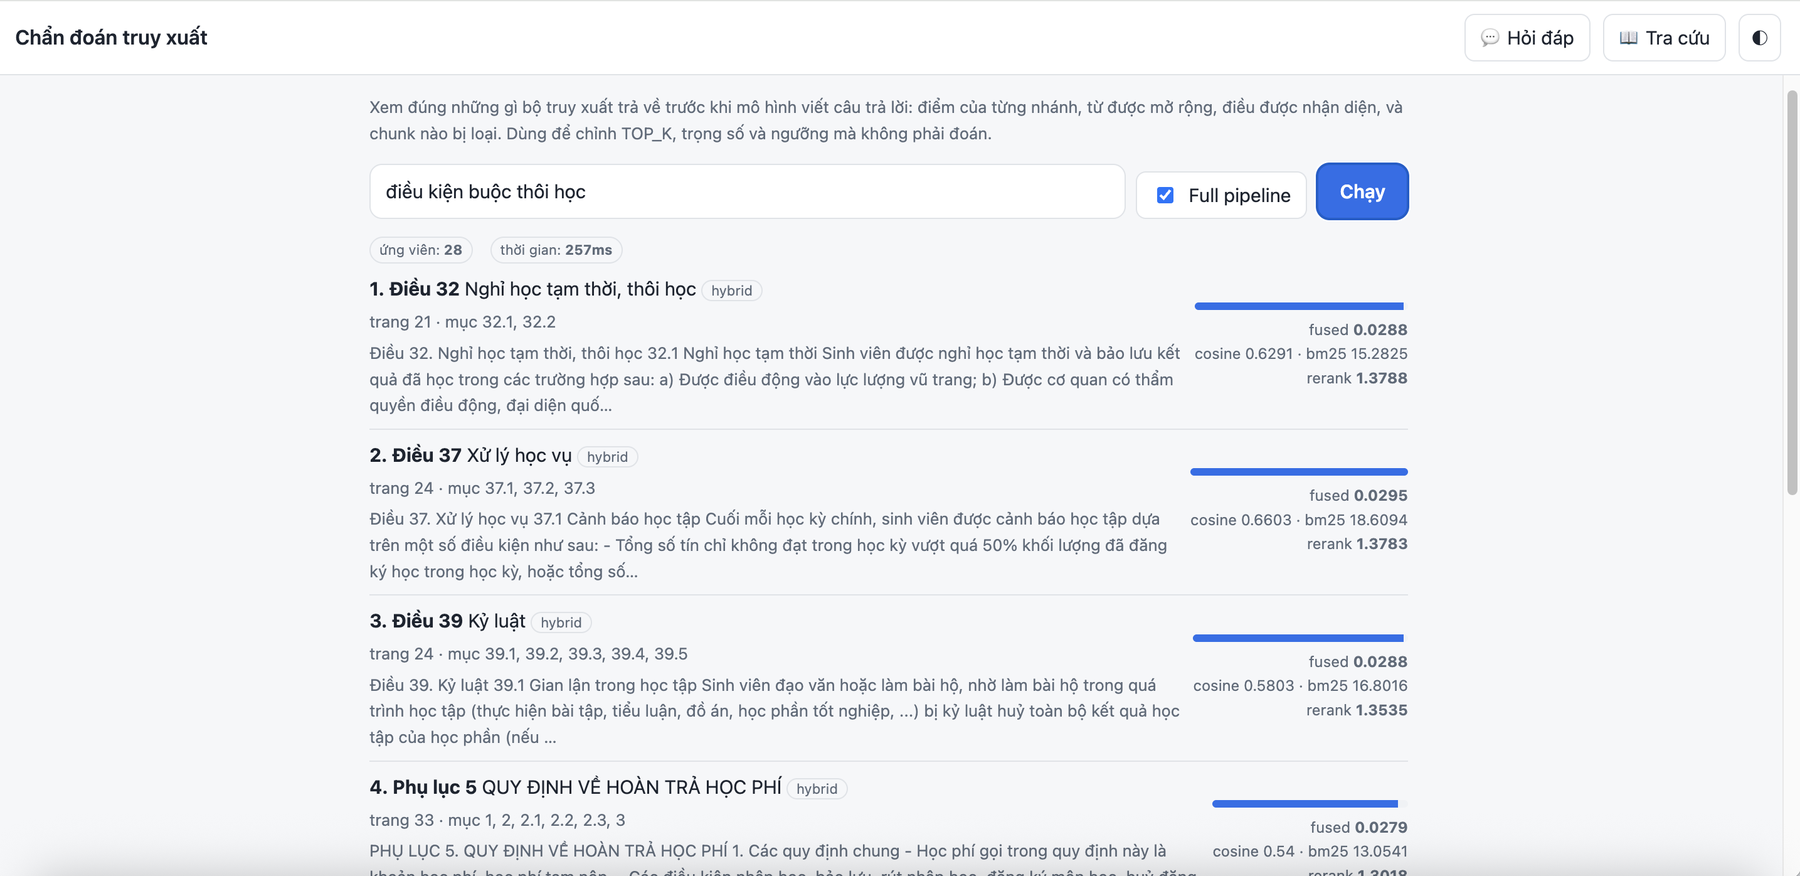
\includegraphics[width=\textwidth]{img/debug-real.png}
\caption{Trang chẩn đoán với câu hỏi “điều kiện buộc thôi học”: 28 ứng viên, 257\,ms, kèm điểm
của từng nhánh cho mỗi chunk.}
\label{fig:debug}
\end{figure}

Điều 37 (Xử lý học vụ) có cosine cao nhất (0,6603) và BM25 cao nhất (18,61), nhưng Điều 32 mới
lên hạng nhất sau rerank — cả hai đều đúng chủ đề. Chính dạng thông tin tách bạch từng nhánh
này cho phép tinh chỉnh trọng số dựa trên quan sát thay vì phỏng đoán.

\subsection{Thống kê kho dữ liệu}

\begin{rtable}
\begin{tabularx}{\textwidth}{@{}X r@{}}
\toprule
\textbf{Chỉ số} & \textbf{Giá trị} \\
\midrule
Số văn bản & 1 \\
Số trang PDF gốc (bản quét, 19\,MB) & 57 \\
Số chương / điều / phụ lục & 10 / 42 / 15 \\
Số chú thích lề tách được & 77 \\
Số chunk sinh ra & 90 \\
Token mỗi chunk: nhỏ nhất / trung vị / lớn nhất & 56 / 508 / 822 \\
Số chunk vượt ngưỡng 800 token (đều là bảng) & 1 \\
Độ dài trung bình (âm tiết mỗi chunk) & 372 \\
Số chunk mang chú thích nguồn gốc & 60 / 90 \\
Số chunk chứa bảng biểu & 18 / 90 \\
\bottomrule
\end{tabularx}
\captionof{table}{Thống kê kho dữ liệu sau khi nạp.}
\label{tab:corpus}
\end{rtable}

Chỉ một chunk vượt ngưỡng token, và đó là một bảng — đúng theo thiết kế, vì bảng không bao giờ
bị cắt. Trung vị 508 token cho thấy phần lớn các Điều vừa trọn trong một chunk.

\subsection{Kết quả đánh giá truy xuất}

Bộ câu hỏi vàng gồm 30 câu trải khắp văn bản, mỗi câu kèm (các) Điều thực sự trả lời được.
Harness bật dần từng kỹ thuật, bắt đầu từ chỉ dùng dense:

\begin{figure}[htbp]
\centering
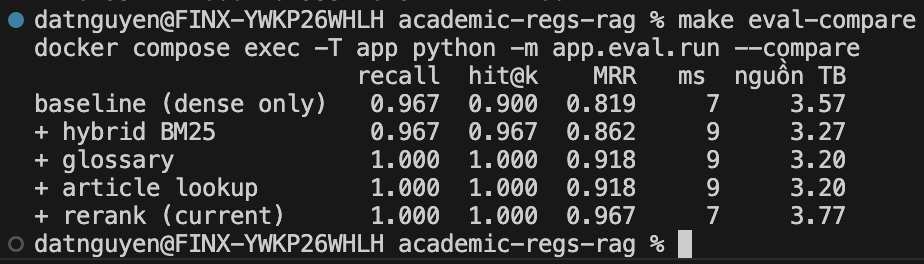
\includegraphics[width=0.84\textwidth]{img/eval-compare.png}
\caption{Kết quả \code{make eval-compare} trên hệ thống thật (bge-m3 + Qdrant), 30 câu hỏi
vàng.}
\label{fig:evalcompare}
\end{figure}

\begin{rtable}
\begin{tabular}{@{}p{0.23\textwidth} r r r r r p{0.22\textwidth}@{}}
\toprule
\textbf{Cấu hình} & \textbf{recall@20} & \textbf{hit@5} & \textbf{MRR} & \textbf{ms}
  & \textbf{nguồn TB} & \textbf{Đóng góp} \\
\midrule
Chỉ dense          & 0,967 & 0,900 & 0,819 & 7 & 3,57 & Nền tảng \\
+ hybrid BM25      & 0,967 & 0,967 & 0,862 & 9 & 3,27 & hit@5 +6,7 điểm \\
+ glossary         & 1,000 & 1,000 & 0,918 & 9 & 3,20 & recall về 100\% \\
+ tra theo số điều & 1,000 & 1,000 & 0,918 & 9 & 3,20 & không đổi trên bộ này \\
\textbf{+ rerank (hiện tại)} & \textbf{1,000} & \textbf{1,000} & \textbf{0,967} & 7 & 3,77
  & MRR +0,049 \\
\bottomrule
\end{tabular}
\captionof{table}{Đóng góp của từng kỹ thuật. \code{recall@20}: Điều đúng có mặt trong danh
sách ứng viên. \code{hit@5}: Điều đúng sống sót qua ngưỡng, rerank và lát cắt cuối. \code{MRR}:
nghịch đảo thứ hạng của Điều đúng. Cột \code{ms} là thời gian truy xuất, không tính lần
embedding đầu tiên vì bộ nhớ đệm đã ấm sau lượt chạy trước.}
\label{tab:eval}
\end{rtable}

Đọc bảng này cho thấy bốn điều mà cảm tính không nói được:

\begin{itemize}
  \item \textbf{BM25 không cải thiện recall mà cải thiện thứ hạng.} Cả hai cấu hình đầu đều tìm
  ra 29/30 Điều đúng ở đâu đó trong 20 ứng viên; khác biệt nằm ở chỗ BM25 đẩy Điều đúng lên đủ
  cao để lọt vào lát cắt cuối (hit@5 từ 0,900 lên 0,967).
  \item \textbf{Bảng thuật ngữ bịt nốt lỗ hổng cuối.} Câu hỏi duy nhất mà hai cấu hình đầu bỏ
  sót là câu gõ không dấu; mở rộng thuật ngữ đưa recall và hit@5 lên 100\%.
  \item \textbf{Tra theo số điều không đóng góp gì trên bộ câu hỏi này}, vì chỉ có một câu gọi
  tên điều khoản và tìm kiếm vector vốn đã tìm ra. Đây là cơ chế \emph{bảo hiểm}: nó bảo đảm
  câu hỏi dạng “Điều 15 nói gì?” không bao giờ hỏng, chứ không phải để nâng điểm trung bình.
  Giữ lại một kỹ thuật không làm tăng điểm là quyết định có ý thức, và bảng đo là thứ cho phép
  đưa ra quyết định đó một cách minh bạch.
  \item \textbf{Rerank đẩy MRR lên 0,967} — gần như lúc nào Điều đúng cũng ở vị trí đầu tiên.
  Với người dùng, điều này quyết định trích đoạn nào được mô hình đọc trước và trích dẫn.
\end{itemize}

\subsubsection{Tinh chỉnh ngưỡng liên quan tương đối}
\label{sec:sweep}

Mục~\ref{sec:nguong} nêu rằng \code{RELATIVE\_CUTOFF} phải đo trên mô hình thật chứ không đoán,
vì siết quá tay sẽ loại nhầm Điều đúng. Harness có chế độ \code{--sweep} in ra chính đường
đánh đổi đó:

\begin{figure}[htbp]
\centering
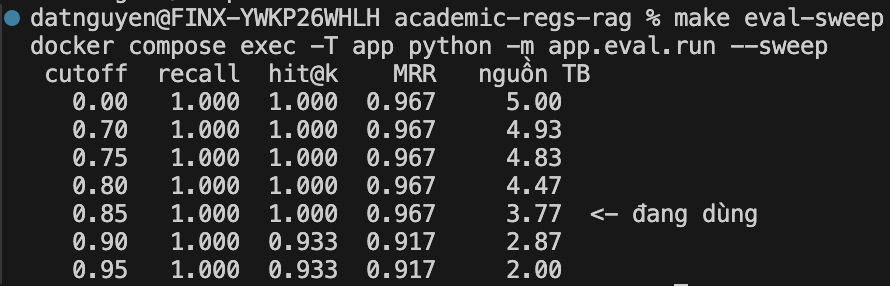
\includegraphics[width=0.80\textwidth]{img/eval-sweep.png}
\caption{\code{make eval-sweep}: số nguồn hiển thị giảm dần khi siết ngưỡng, và điểm gãy nằm ở
0,90.}
\label{fig:evalsweep}
\end{figure}

\begin{rtable}
\begin{tabular}{@{}r r r r r p{0.36\textwidth}@{}}
\toprule
\textbf{cutoff} & \textbf{recall} & \textbf{hit@5} & \textbf{MRR} & \textbf{nguồn TB}
  & \textbf{Nhận xét} \\
\midrule
0,00 & 1,000 & 1,000 & 0,967 & 5,00 & Không lọc: luôn trả đủ định mức \\
0,70 & 1,000 & 1,000 & 0,967 & 4,93 & Gần như không lọc được gì \\
0,75 & 1,000 & 1,000 & 0,967 & 4,83 & \\
0,80 & 1,000 & 1,000 & 0,967 & 4,47 & \\
\textbf{0,85} & \textbf{1,000} & \textbf{1,000} & \textbf{0,967} & \textbf{3,77}
  & \textbf{Đang dùng: bớt 25\% số nguồn mà không mất gì} \\
0,90 & 1,000 & 0,933 & 0,917 & 2,87 & Điểm gãy: bắt đầu loại nhầm Điều đúng \\
0,95 & 1,000 & 0,933 & 0,917 & 2,00 & Quá chặt \\
\bottomrule
\end{tabular}
\captionof{table}{Đường đánh đổi của \code{RELATIVE\_CUTOFF} trên 30 câu hỏi vàng.}
\label{tab:sweep}
\end{rtable}

Kết quả cho thấy giá trị 0,85 là \textbf{miễn phí}: \code{hit@5} và \code{MRR} giữ nguyên hệt
như khi không lọc, trong khi số trích đoạn trung bình đưa ra cho người đọc giảm từ 5,00 xuống
3,77 — tức một phần tư số “nguồn tham khảo” trước đây là phần đệm không đóng góp gì. Điểm gãy
nằm ở 0,90, nơi \code{hit@5} tụt xuống 0,933. Đây đúng là dạng quyết định mà nếu không có công
cụ đo thì chỉ còn cách chọn bừa một con số rồi hy vọng.

\subsection{Kiểm thử tự động}

\begin{rtable}
\begin{tabular}{@{}p{0.24\textwidth} r p{0.55\textwidth}@{}}
\toprule
\textbf{Tệp} & \textbf{Test} & \textbf{Kiểm tra điều gì} \\
\midrule
\code{test\_chunk.py} & 9 & Mọi Điều/Phụ lục đều có chunk; chỉ bảng được vượt ngưỡng; mã chunk tất định \\
\code{test\_retriever.py} & 17 & Hợp nhất giữ điểm từng nhánh; tra theo số điều; ngưỡng liên quan; mở rộng lân cận; số nguồn biến thiên \\
\code{test\_chat.py} & 14 & Thứ tự sự kiện SSE; đường từ chối; soát trích dẫn; bộ bảo vệ rewrite \\
\code{test\_api.py} & 10 & Mục lục, đọc Điều, cấu hình không lộ khoá, chống path traversal \\
\code{test\_glossary.py} & 7 & Viết tắt, tiếng lóng, không dấu, viết tắt 2 ký tự phải hoa \\
\code{test\_rerank.py} & 7 & IDF cục bộ; độ phủ; chunk hạng thấp được nâng lên; phạt trùng Điều \\
\code{test\_citations.py} & 5 & Bắt số Điều/khoản/Phụ lục; phát hiện trích dẫn vô căn cứ \\
\midrule
\textbf{Tổng} & \textbf{69} & Chạy trong khoảng một giây, không cần Ollama, Qdrant hay mạng \\
\bottomrule
\end{tabular}
\captionof{table}{Bộ kiểm thử tự động.}
\label{tab:tests}
\end{rtable}

Việc bộ test chạy được mà không cần hạ tầng là một quyết định thiết kế chứ không phải tiện lợi
ngẫu nhiên: Qdrant có chế độ in-memory, và embedder được thay bằng một bộ băm túi từ tất định.
Bộ test nào cần dựng cả stack mới chạy được thì sẽ không ai chạy.

\subsection{Hiệu năng}

\begin{rtable}
\begin{tabularx}{\textwidth}{@{}X r@{}}
\toprule
\textbf{Giai đoạn} & \textbf{Thời gian đo được} \\
\midrule
Truy xuất (hybrid + rerank + mở rộng) & 11 – 340\,ms \\
Toàn bộ một lượt hỏi đáp (gpt-4o-mini) & 2,4 – 6,1\,s \\
Lượt bị từ chối (không gọi mô hình sinh) & 1,3\,s \\
Nạp dữ liệu lại toàn bộ 90 chunk (CPU) & vài phút \\
Nạp dữ liệu khi không có thay đổi & tức thì \\
\bottomrule
\end{tabularx}
\captionof{table}{Hiệu năng đo trên máy thật, chế độ cloud (\code{--cloud}, embedding vẫn
chạy local).}
\label{tab:perf}
\end{rtable}

Độ trễ tổng bị chi phối hoàn toàn bởi bước sinh câu trả lời; phần truy xuất chiếm chưa tới
10\%. Đây là lý do việc gửi trích đoạn trước token đầu tiên (mục~\ref{sec:latency}) có giá trị
thực tế: người đọc nhận được nội dung kiểm chứng được sau khoảng 300\,ms, thay vì phải chờ hết
vài giây.

\chapterbreak
